\documentclass{standalone}
\usepackage{tikz}
\usepackage{mathtools}
\usepackage{pgfplots}

\pgfplotsset{compat=newest}

\begin{document}
    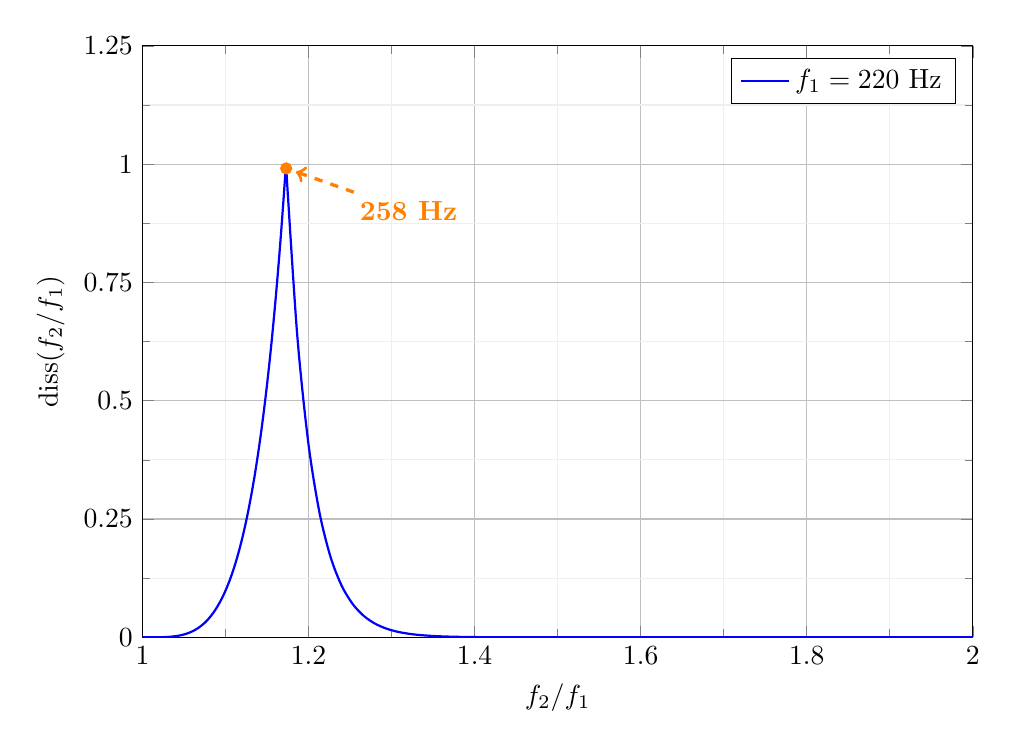
\begin{tikzpicture}
        \begin{axis}[
            xmin = 1, xmax = 2, %
            ymin = 0, ymax = 1.25, %
            xtick distance = 0.2, %Is the distance between major ticks in the x-axis.
            ytick distance = 0.25, %Is the distance between major ticks in the y-axis.
            grid = both, %When this options is set to both the minor and major grid are plotted.
            minor tick num = 1, %Is the number of ticks between major ticks.
            major grid style = {lightgray}, %Changes the color and stroke of the major grid.
            minor grid style = {lightgray!25}, %Changes the color and stroke of the minor grid.
            width = \textwidth, %sets the width of the figure
            height = 0.75\textwidth,  %sets the height of the figure
            xlabel = {$f_2/f_1$}, %
            ylabel = {$\text{diss}(f_2/f_1)$}, %
            legend cell align = {left}, %
        ]
            %%%%%%%%%%%%%%%% Frequency2 %%%%%%%%%%%%%%%%
            \addplot[
                domain=1:1.1727, %Domain of the fucntion
                samples=100, %This parameter determines the number of point to be plotted for the function, while bigger the number better looks the function.
                smooth, %f we use this option, the compiler makes an interpolation between the point plotted to get a soft appearance for the function.
                thick, %Stroke of the function. Options: ultra thin, very thin, thin, semithick, thick, very thick, ultra thick.
                blue %Color of the function.
            ]{cosh(44.14273*(x-1)^2)-1};
            \addplot[
                domain=1.1727:2.5, %Domain of the fucntion
                samples=100, %This parameter determines the number of point to be plotted for the function, while bigger the number better looks the function.
                smooth, %f we use this option, the compiler makes an interpolation between the point plotted to get a soft appearance for the function.
                thick, %Stroke of the function. Options: ultra thin, very thin, thin, semithick, thick, very thick, ultra thick.
                blue %Color of the function.
            ]{exp(-0.15*220*(x-1-38/220)};
            \node [anchor=west,color=orange,font=\bf] (freq) at (axis cs:1.25,0.9){258 Hz}; 
            \node (disso) at (axis cs:1.173,0.991){};
            \draw[->,color=orange,very thick,dashed](freq)--(disso);
            \addplot [mark=oplus*,mark size=2pt,orange] coordinates {(1.173,0.991)};
            \legend{$f_1=220\text{ Hz}$}
        \end{axis}
    \end{tikzpicture}
\end{document}